% The next command tells RStudio to do "Compile PDF" on HSB.Rnw,
% instead of this file, thereby eliminating the need to switch back to HSB.Rnw 
% before building the paper.
%!TEX root = ../HSB.Rnw

\renewcommand{\arraystretch}{0.6}

\begin{landscape}
\begin{table}
\begin{center}
\caption{Comparison among relevant rebound analysis frameworks.}
\begin{tabular}{r c c c c c c}
  \toprule
                                             & \rot{\citet{Nassen:2009aa}}
                                             & \rot{\citet{Thomas:2013aa}}
                                             & \rot{\citet{Chan2015}}
                                             & \rot{\citet{Borenstein:2015aa}}
                                             & \rot{\citet{Wang2021}}
                                             & \rot{This paper} \\
  \midrule
  % \multicolumn{1}{l}{\emph{Integrated effects, locations, and scales}}    &          &                &                &                 &                &\\
  \emph{Integrated effects, locations, and scales}                &          &                &                &                 &                &\\
  Direct emplacement effect                                       & ?\rating{50}     & \rating{0}    & \rating{00}    & \rating{00}    & ?\rating{0}   & \rating{100}      \\
  Embodied energy effect                                          & \rating{0}     & \rating{0}    & \rating{00}    & \rating{50}    & ?\rating{0}   & \rating{100}   \\
  Maintenance and disposal effect                                 & ?\rating{25}     & \rating{0}    & \rating{00}    & ?\rating{0}    & ?\rating{0}   & \rating{100}   \\
  Direct substitution effect                                      & \rating{50}     & \rating{50}    & \rating{100}    & \rating{100}    & \rating{100}   & \rating{100}   \\
  Indirect substitution effect                                    & \rating{50}     & \rating{50}    & \rating{100}    & \rating{100}    & \rating{100}   & \rating{100}   \\
  Direct income effect                                            & \rating{50}     & \rating{50}    & \rating{100}    & \rating{100}    & \rating{100}   & \rating{100}   \\
  Indirect income effect                                          & \rating{50}     & \rating{50}    & \rating{100}    & \rating{100}    & \rating{100}   & \rating{100}   \\
  Macro effect                                                    & \rating{0}     & \rating{0}    & \rating{0}    & \rating{25}    & \rating{0}   & \rating{100}   \\
  \midrule
  Analyses in energy, expenditure, and consumption spaces         & ?\rating{50}     & ?\rating{75}    & ?\rating{75}    & \rating{50}    & ?\rating{50}   & \rating{100}   \\
  Detailed model of consumer preferences                          & \rating{25}     &  \rating{50}   & \rating{100}    & \rating{50}    & \rating{100}   & \rating{100}\\
  Non-marginal energy service price changes                       & ?\rating{0}     &  \rating{0}   & ?\rating{0}    & \rating{0}    & \rating{0}   & \rating{100}\\
  Operationalizable                                               & \rating{100}     &  \rating{100}   & \rating{0}    & \rating{50}    & \rating{0}   & \rating{100}\\
\bottomrule
\end{tabular}
\label{tab:previous_frameworks}
\end{center}
\end{table}
\end{landscape}

% \renewcommand{\arraystretch}{1}

% \begin{table} 
%   \caption{Previous rebound analysis frameworks. **** This table is not correct. We need to decide which 
%            frameworks to include and their characteristics. ---MKH ****}
%   \centering
%   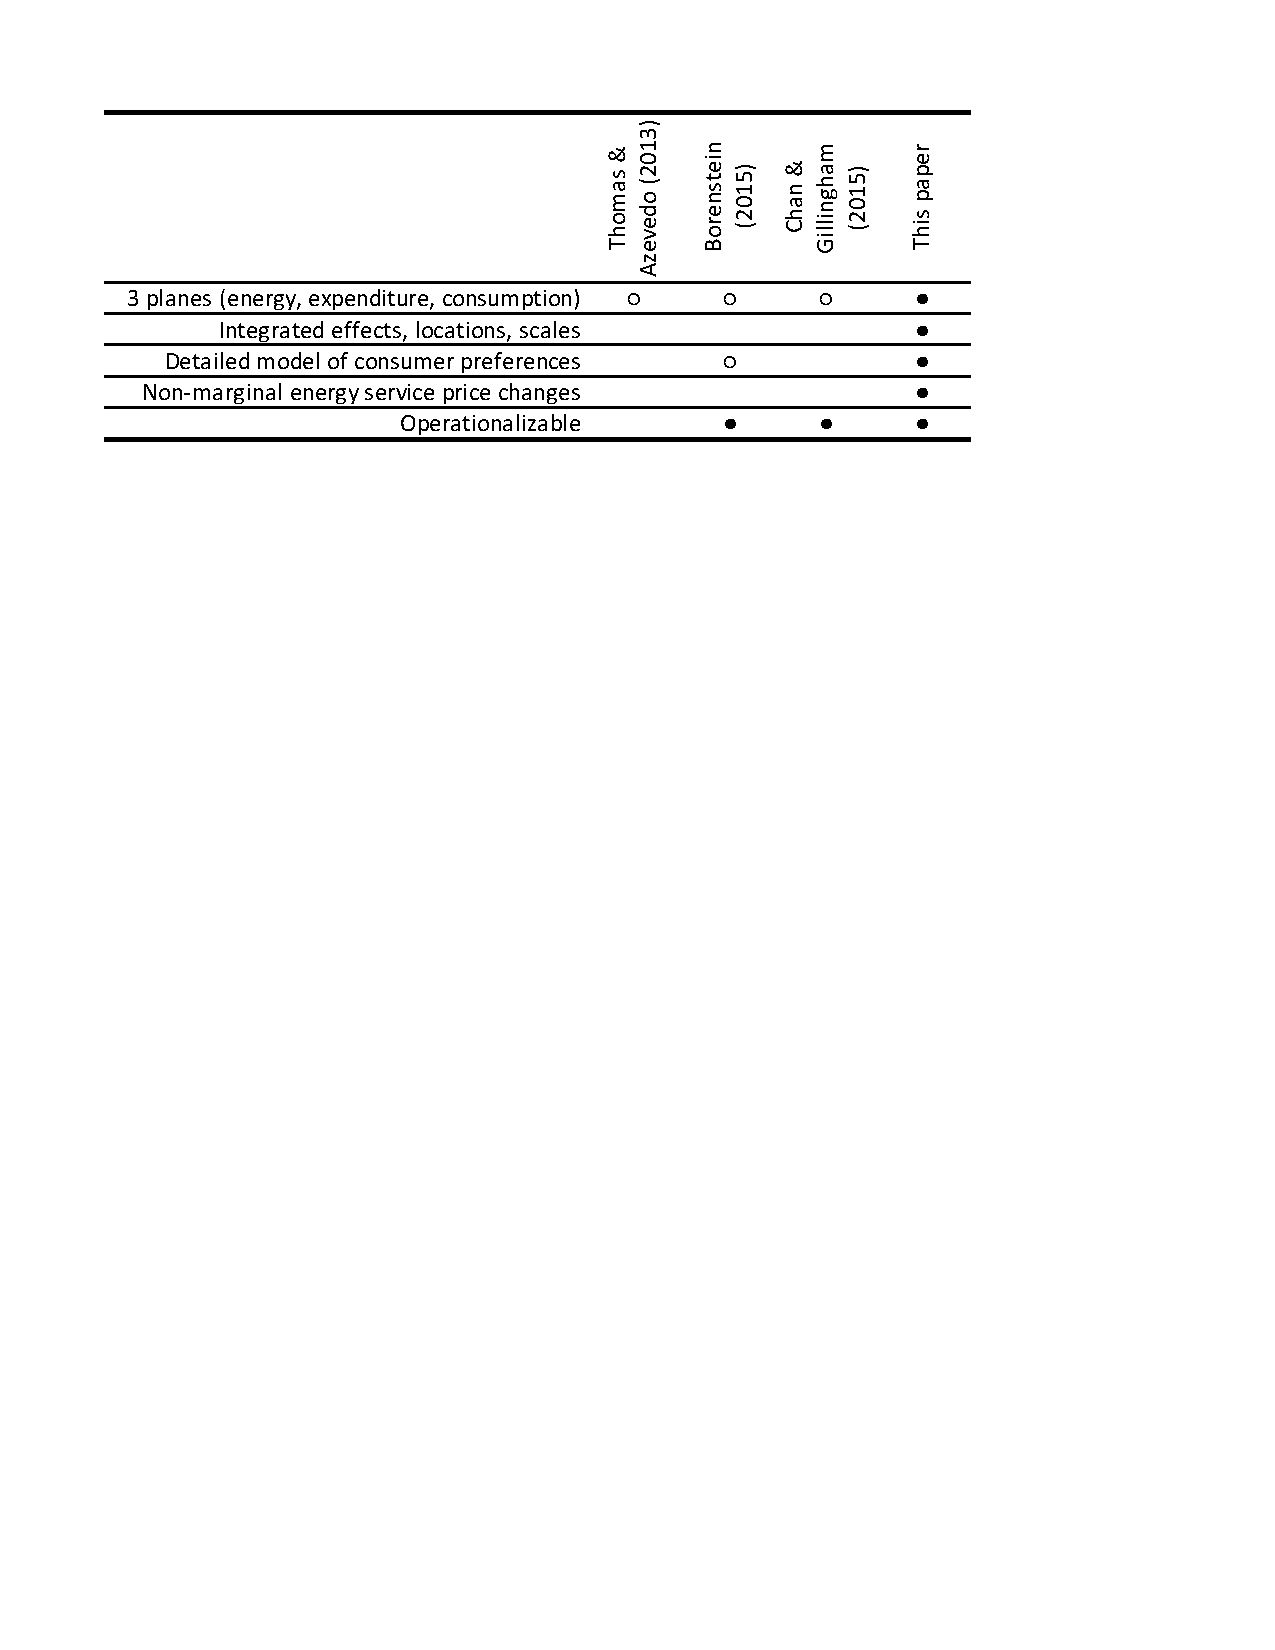
\includegraphics[width=1\linewidth]{figure_other/PreviousFrameworksTable.pdf}
%   \label{tab:previous_frameworks}
% \end{table}

